%% Alban Kraus
%% © 2016 École nationale des sciences géographiques
%% 6-8 avenue Blaise Pascal - Champs-sur-Marne
%% 77455 MARNE-LA-VALLÉE CEDEX 2

\documentclass[a4paper, oneside, twocolumn, 12pt]{report}

% Directories
\newcommand\fragment{fragment}
\newcommand\data{data}

% French typesetting
\usepackage[utf8]{inputenc}
\usepackage[T1]{fontenc}
\usepackage[english, french]{babel}
\usepackage{numprint}
\usepackage{lmodern}

% Meta-data
\usepackage{color}
\usepackage[
  hyperindex=true,
  bookmarks=true,
  baseurl={https://github.com/alkra/MPIMP},
  pdftitle={Rapport des TP de parallélisation},
  pdfauthor={Alban Kraus},
  pdfsubject={Parallélisation -- mars 2016},
  pdfproducer={École nationale des sciences géographiques -- 6-8 avenue Blaise Pascal - Champs-sur-Marne -- 77455 MARNE-LA-VALLÉE CEDEX 2},
  pdflang=fr-FR
]{hyperref}

\title{Rapport des TP de parallélisation}
\author{Alban Kraus}
\date{23 mars 2016}

% Headings customization
\usepackage{titlesec}

\newcounter{question}
\renewcommand\thesubsection{Q.~\arabic{question}}
\titleformat{\subsection}[hang]{\normalfont\large\bfseries}{Question~\arabic{question}}{0.7em}{}{}
\newcommand\question{\subsection{}}
\titleformat{\chapter}[display]{\normalfont\huge\bfseries\centering}{TP~\thechapter}{20pt}{\Huge}

% Other packages (style - maths - graphics)
\usepackage{framed}
\usepackage{longtable}
\usepackage{tabularx}
\usepackage{array}
\usepackage{amsmath}
\usepackage[scientific-notation=true]{siunitx}
\usepackage{pgfplots}
\pgfplotsset{compat=1.11}
\pgfplotsset{width=7.5cm}
\usepackage{tikz}
\usepackage{transparent}
\usepackage{graphicx}
\usepackage{eso-pic}

% First page's overlay
\newcommand\BackgroundPic{%
  \put(0, 0){%
    \parbox[b][\paperheight]{\textwidth}{%
      \transparent{0.3}%
      \vfill%
      \centering%
      \lstset{%
        basicstyle=\footnotesize,
        showspaces=false
      }%
      \lstinputlisting[language=C, firstline=217, lastline=391]{\fragment/mandel.c}%
      \vfill%
    }%
  }%
}

% Code
\usepackage{listings}
\definecolor{comments}{gray}{0.7}
\definecolor{keywords}{rgb}{0.1, 0.1, 0.9}
\definecolor{strings}{rgb}{0.8, 0.05, 0.7}
\lstset{
  commentstyle=\color{comments}\rmfamily,
  keepspaces=true,
  keywordstyle=\color{keywords},
  stringstyle=\color{strings}
}

\usepackage[french, longend, ruled]{algorithm2e}
% Constantes
\SetKwData{MASTER}{MAÎTRE}

% Entrées / sorties
\SetKwInput{Variables}{Variables locales}
\SetKwData{H}{h}
\SetKwData{W}{w}
\SetKwData{P}{nproc}
\SetKwData{Rank}{rank}
\SetKwData{Hlocal}{h\_local}
\SetKwData{Ima}{ima}
\SetKwData{Pima}{pima}
\SetKwData{Xmin}{xmin}
\SetKwData{Xmax}{xmax}
\SetKwData{Ymin}{ymin}
\SetKwData{Ymax}{ymax}
\SetKwData{Xincr}{xincr}
\SetKwData{Yincr}{yincr}
\SetKwData{Filtre}{filtre}
\SetKwData{Niter}{nbiter}
\SetKwData{R}{r}

% fonctions C
\SetKwFunction{sizeof}{sizeof}
\SetKwFunction{malloc}{malloc}

% fonctions MPI
\SetKwData{CommWorld}{MPI\_COMM\_WORLD}
\SetKwData{Char}{MPI\_CHAR}
\SetKwData{Int}{MPI\_INT}
\SetKwFunction{Recv}{MPI\_Recv}
\SetKwFunction{Send}{MPI\_Send}
\SetKwFunction{Bcast}{MPI\_Bcast}
\SetKwFunction{Scatter}{MPI\_Scatter}
\SetKwFunction{Gather}{MPI\_Gather}
\SetKwData{AnySource}{MPI\_ANY\_SOURCE}
\SetKwFunction{Probe}{MPI\_Probe}
\SetKwData{Source}{MPI\_SOURCE}
\SetKwData{Exchange}{TAG\_LINE\_EXCHANGE}

% Style
\DontPrintSemicolon









%%%%%%%%%%%%
% DOCUMENT %
%%%%%%%%%%%%


\begin{document}

% Title page
\twocolumn[
\begin{@twocolumnfalse}
  \newlength\ensg
\settowidth\ensg{\small 6-8 avenue Blaise Pascal -- Champs-sur-Marne}

\begin{titlepage}

  % Background picture
  \AddToShipoutPicture*{\BackgroundPic}

  % ENSG
  \begin{flushright}
    \begin{tabular}{p{\ensg} p{0.25\textwidth}}
      {%
      \small
      ~\newline
      École nationale des sciences géographiques

      6-8 avenue Blaise Pascal -- Champs-sur-Marne\newline
      77455 MARNE-LA-VALLÉE CEDEX 2
      } & \raisebox{-0.9\height}[0pt][0.8\height]{%
          
\includegraphics[width=0.25\textwidth]{\fragment/logo_ensg}%
          } \\
    \end{tabular}
  \end{flushright}

  % Titles
  \begin{center}
    \vskip 0.1\textheight

    \begin{framed}
      \bigskip

      \Huge\sffamily\bfseries
      Rapport des travaux pratiques

      \bigskip

      \LARGE\rmfamily\mdseries
      Cours de parallélisation

      de Ahmad \bsc{Audi}

      \bigskip
    \end{framed}

    \vskip 0.1\textheight

    \bfseries\Large
    Alban Kraus
    
    \smallskip

    \normalsize\mdseries
    Cycle ingénieur, promotion 2013

    \vskip 0.18\textheight

    23 mars 2016
  \end{center}
\end{titlepage}


%%% Local Variables:
%%% mode: latex
%%% TeX-master: "rapport"
%%% End:

\end{@twocolumnfalse}
]

\clearpage

% Copyright notice
\thispagestyle{empty}
\twocolumn[
\begin{@twocolumnfalse}
  \vskip 0.8\textheight

  \begin{minipage}{\textwidth}
  \centering\footnotesize
  Cette œuvre est protégée en France et dans d'autre pays.
  
  \bigskip

  
\includegraphics{\fragment/CC-BY}
    
  \bigskip

  Vous pouvez réutiliser cette œuvre selon les termes de la licence

  \href{https://creativecommons.org/licenses/by/3.0/deed.fr}{%
    Creative commons -- attribution 3.0 non transposé}
\end{minipage}


%%% Local Variables:
%%% mode: latex
%%% TeX-master: "../rapport"
%%% End:

\end{@twocolumnfalse}
]

\clearpage

\tableofcontents


% TP 1

\chapter{Ensemble de Mandelbrot}

\setcounter{question}{0}
\loop\ifnum\arabic{question}<5
\stepcounter{question}
\input{mandelbrot/question-\arabic{question}}
\repeat

% TP 2

\chapter{Convolution}

%% Alban Kraus
%% © 2016 École nationale des sciences géographiques
%% 6-8 avenue Blaise Pascal - Champs-sur-Marne
%% 77455 MARNE-LA-VALLÉE CEDEX 2

\section{Questions liminaires}

\subsubsection{La fonction convolution}

\begin{quotation}
  Dans la fonction \texttt{con\-vo\-lu\-tion(\-)}, pourquoi doit-on
  préparer un tampon intermédiaire au lieu de faire le calcul
  directement sur l'image ?
\end{quotation}

Le filtre s'applique à plusieurs pixels de l'image \emph{originale}
(ou de la convolution $i-1$). Si on fait le calcul directement sur
l'image (convolution $i$), il y aura au moins un de ces pixels qui
aura été altéré par le calcul précédent.

On a alors besoin de deux tampons : l'un contient l'image originale,
et l'autre l'image convoluée. À la fin du calcul, on remplace l'image
originale par l'image convoluée, qui sera l'image originale de la
prochaine convolution.


\subsubsection{Parallélisation de l'algorithme}

\begin{quotation}
  Quelles sont les séquences parallélisables de l'algorithme ?
\end{quotation}

Le calcul de la convolution ne dépend que de l'image originale : il
peut donc \^etre parallélisé. Autrement dit, le calcul de chaque pixel
est indépendant.

L'application du filtre ne peut pas \^etre parallélisée en règle
générale.

De plus, la composition des convolutions ne peut pas \^etre
parallélisée, car chacune dépend de la précédente.



\subsubsection{Équilibrage de charge}

\begin{quotation}
  Sachant que la taille du noyau $k$ de convolution est $3 \times 3$
  pixels, quelle est la complexité théorique du calcul d'un pixel de
  $I * k$ ? Quel type d'équilibrage de charge doit-on prévoir entre
  les processeurs ?
\end{quotation}

Pour chaque pixel, l'application du filtre se fait en temps constant
(ne dépend que de la taille du filtre). On peut donc appliquer une
répartition statique de charge.


\subsubsection{Découpage}

\begin{quotation}
  Quel découpage (répartition des données entre processeurs) est
  naturel dans ce contexte ?
\end{quotation}

Afin de minimiser les communications entre processus, et aussi parce
qu'il est plus simple à mettre en place, nous allons réaliser un
découpage en \emph{lignes}.


\subsubsection{Problèmes aux bords}

\begin{quotation}
  Quel problème (au bord des blocs de l'image) survient lors de
  l'itération de l'opération de convolution ?
\end{quotation}

Lors du calcul d'un bloc de l'image, chaque processus aura besoin de
la dernière ligne du processus précédent et de la première du suivant
pour calculer sa première ligne et sa dernière.

Chaque processus doit ainsi communiquer sa première ligne au processus
précédent et sa dernière ligne au processus suivant.


\subsubsection{Pseudo-code}

\begin{quotation}
  Implémenter un algorithme parallèle avec des envois bloquants de
  message.
\end{quotation}

\begin{algorithm}[t]
  \caption{Lecture de l'image}
  \label{alg:convol:stat:file}
  \Donnees{\;
    \begin{tabular}{l @{ : } l}
      \Rank & rang du processus (connu)\\
    \end{tabular}
  }

  \Variables{\;
    \begin{tabularx}{\linewidth}{l @{ : } X}
      $params$ & tableau [2] contenant les tailles des images\\
    \end{tabularx}
  }

  \Res{\;
    \begin{tabular}{l @{ : } l}
      \R & fichier image\\
      \H & hauteur de l'image\\
      \W & largeur de l'image\\
    \end{tabular}
  }

  \Deb{%
    \Si{\Rank == \MASTER}{%
      Lecture du fichier\;
      Récupération de $params$\;
    }

    \tcp{Envoi des paramètres}
    \hangindent=\skiptext\hangafter=1
    \Bcast{$params$, 2, \Int, \MASTER, \CommWorld}\;
    \H = $params$[0]\;
    \W = $params$[1]\;
  }
\end{algorithm}

Les algorithmes \ref{alg:convol:stat:file} et
\ref{alg:convol:stat:mem} ne nécessitent que peu d'explications. Le
processus maître lit l'image et l'envoie à ses esclaves. La fonction
\texttt{MPI\_Scatter} se charge de répartir statiquement la charge de
travail entre les processus esclaves.

Néanmoins, comme établi à la question précédente, cet envoi ne
concerne que les lignes propres au processus en question. Les échanges
de lignes se déroulent dans l'algorithme \ref{alg:convol:stat:calc}.

\begin{algorithm*}
  \caption{Allocation de la mémoire}
  \label{alg:convol:stat:mem}

  \Donnees{\R, \H, \W, \Rank\;
    \begin{tabular}{l @{ : } l}
      \P & nombre de processus (connu)\\
    \end{tabular}
  }

  \Res{\;
    \begin{tabularx}{\linewidth}{l @{ : } X}
      \Hlocal & hauteur d'un bloc\\
      \Ima & pointeur vers le début de l'image\\
    \end{tabularx}
  }

  \Deb{
    \hangindent=\skiptext\hangafter=1
    \Hlocal = \H / \P \\
    + (\Rank > 0 ? 1 : 0)\\
    + (\Rank < \P-1 ? 1 : 0)\;

    \uSi{\Rank == \MASTER}{
      \Ima = \R.data;
    }
    \Sinon{
      \hangindent=\skiptext\hangafter=1
      \Ima = \malloc{\Hlocal * \W * \sizeof{unsigned char}}\;
      Test de l'allocation\;
    }

    \hangindent=\skiptext\hangafter=1
    \Scatter{
      \Ima, \mbox{\W * \H / \P, \Char},
      \mbox{\Ima + (\Rank > 0 ? \W : 0)},
      \mbox{\W * \H / \P}, \Char, \MASTER, \CommWorld
    }\;
  }
\end{algorithm*}

Chaque processus différent du premier commence par envoyer sa deuxième
ligne au précédent. Pour éviter un blocage perpétuel, le deuxième
\texttt{if} doit commencer par la réception de la dernière
ligne. Explications dans le tableau \ref{tab:convol:stat:bloquant}.

Une fois l'échange de lignes effectué, le travail peut
commencer. Entre chaque application du filtre, les processus échangent
à nouveau leurs lignes extrêmes, car elles ont été modifiées.

À la fin du calcul, tous les processus envoient leur résultat sans la
première ni la dernière ligne, et \texttt{MPI\_Gather} se charge de
refabriquer l'image finale.

\begin{table*}
  \centering
  \begin{tabularx}{\linewidth}{X X X X}
    Processus 0 & Processus 1 & Processus 2 & Processus 3\\
    \hline
    Recv(1) \hfill $\leftarrow$  & Send(0)   & Send(1)     & Send(2)\\
    Send(1) \hfill $\rightarrow$ & Recv(0)   & Send(1)     & Send(2)\\
    \hline
    (travail) & Recv(2) \hfill $\leftarrow$  & Send(1)   & Send(2)\\
              & Send(2) \hfill $\rightarrow$ & Recv(1)   & Send(2)\\
    \hline
              & (travail) & Recv(3) \hfill $\leftarrow$  & Send(2)\\
              &           & Send(3) \hfill $\rightarrow$ & Recv(3)\\
    \hline
              &           & (travail)             & (travail)\\
  \end{tabularx}
  \caption{Échange bloquant des lignes}
  \label{tab:convol:stat:bloquant}
\end{table*}

\begin{algorithm*}
  \caption{Calcul et envoi du résultat}
  \label{alg:convol:stat:calc}

  \Donnees{\Ima, \W, \H, \Hlocal, \Rank, \P\;
    \begin{tabular}{l @{ : } l}
      \Filtre & numéro du filtre (commande)\\
      \Niter & nombre d'itérations (commande)\\
    \end{tabular}
  }

  \Variables{\;
    \begin{tabular}{l @{ : } l}
      $status$ & état de la requête\\
      $i$ & itération courante\\
    \end{tabular}
  }

  \Deb{%
    \Pour{$i$ de 0 à \Niter} {
      \tcp{Communications avec le processus précédent}
      \Si{\Rank > 0}{
        \Send{\Ima + \W, \W, \Char, \Rank-1, \Exchange, \CommWorld}\;
        \Recv{\Ima, \W, \Char, \Rank-1, \Exchange, \CommWorld,
          \&$status$}\;
      }

      \tcp{Communications avec le processus suivant}
      \Si{\Rank < \P-1}{
        \Recv{%
          \mbox{\Ima + (\Hlocal-1) * \W},
          \W, \Char, \Rank+1, \Exchange, \CommWorld, \&$status$
        }\;
        \Send{%
          \mbox{\Ima + (\Hlocal-2) * \W},
          \W, \Char, \Rank+1, \Exchange, \CommWorld
        }\;
      }

      calcul(\Filtre, \Ima, \Hlocal, \W)\;
    }

    \Gather{%
      \mbox{\Ima+\W},
      \mbox{\W * \H / \P}, \Char, \Ima,
      \mbox{\W * \H / \P}, \Char, \MASTER, \CommWorld
    }\;

    \Si{\Rank == \MASTER}{%
      Enregistrement de \Ima\;
    }
  }
\end{algorithm*}

\subsubsection{Analyse des performances}

Les tests ont été effectués sur l'image Albert-Einstein.ras en figure
\ref{fig:convol:einstein}, dont la provenance est douteuse. Cette
image a pour dimensions $1200 \times 1000$.

\begin{figure}
  \centering
  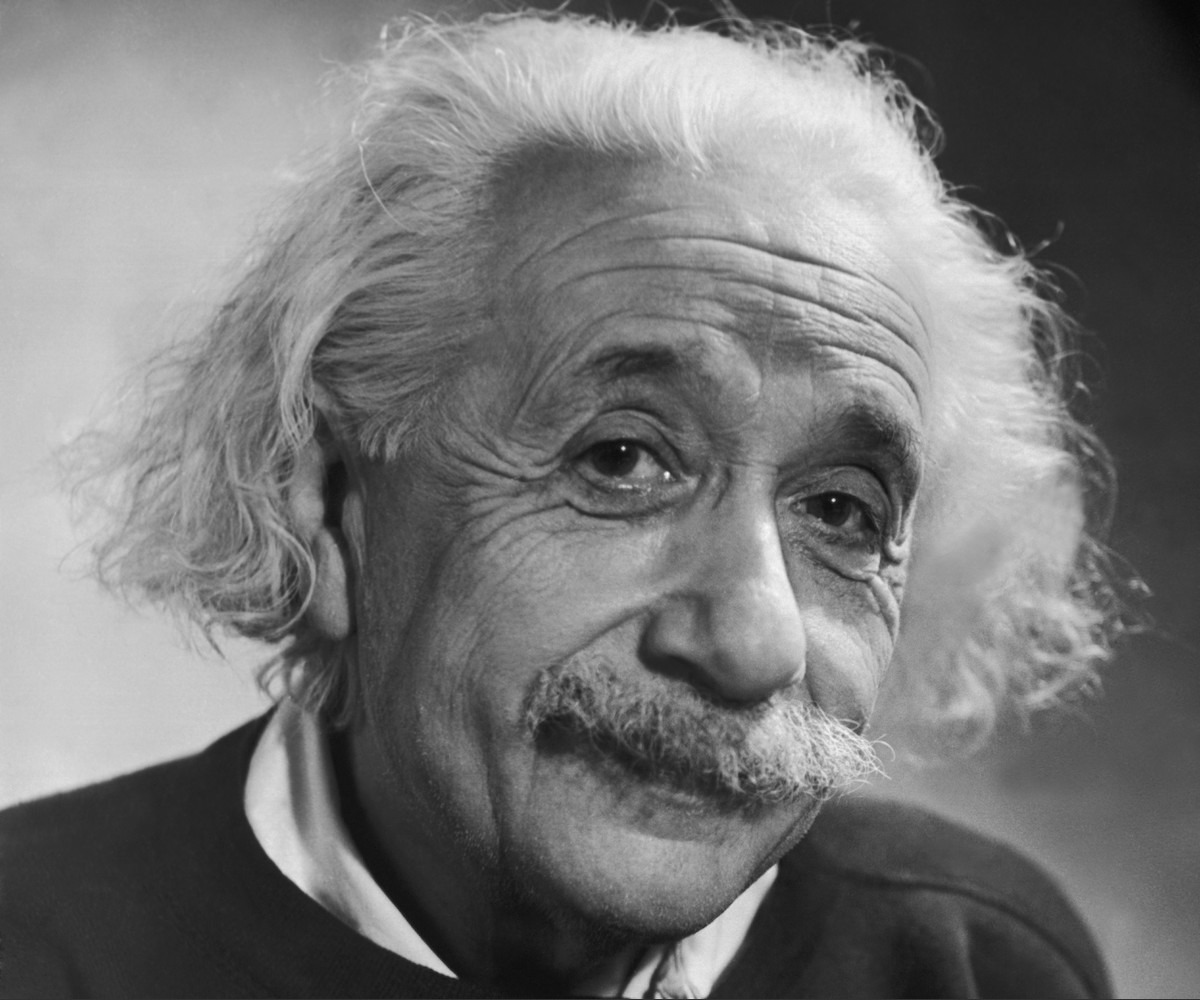
\includegraphics[width=\linewidth]{\fragment/Albert-Einstein}
  \caption{L'image de test}
  \label{fig:convol:einstein}
\end{figure}

Dans la figure \ref{fig:convol:iter}, on s'intéresse aux performances
de calcul en fonction du nombre d'itérations. Le filtre 4 est beaucoup
plus long à appliquer que les autres ; il fait donc l'objet d'un
diagramme séparé.

\paragraph{Le filtre 4}
Toutes les courbes sont linéaires et s'intersectent en $(0, 0)$. On
peut donc en lire la pente aisément : avec six machines, le filtre 2
a une pente de 4 secondes par millier d'itérations, et le filtre 4 de
120 secondes par millier d'itérations. La pente du filtre 4 est donc
trente fois plus grande que celle des autres filtres. Le tri des
valeurs pour en extraire la médiane peut être une source de calculs
supplémentaires ; pour valider cette hypothèse, il serait nécessaire
d'examiner le code assembleur et compter les opérations, ce qui me
paraît trop compliqué pour le cadre de ce TP.

\begin{figure}
  \centering

  \begin{tikzpicture}
    \begin{axis}[
      xlabel={Nombre d'itérations},
      ylabel={Temps de calcul (s)},
      legend style={
        at={(0.5,1)},
        anchor=south
      }
      ]

      \addplot[red, dashed] table [x index=3, y index=4,
      col sep=semicolon, header=false]{%
        \data/convol-iter-1-4.csv%
      };

      \addplot[red] table [x index=3, y index=4,
      col sep=semicolon, header=false]{%
        \data/convol-iter-6-4.csv%
      };

      \legend{filtre 4 (1 machine), filtre 4 (6 machines)}
    \end{axis}
  \end{tikzpicture}

  \begin{tikzpicture}
    \begin{axis}[
      xlabel={Nombre d'itérations},
      ylabel={Temps de calcul (s)},
      legend style={
        at={(0.5,1)},
        anchor=south
      }
      ]
      \addplot[black, dashed] table [x index=3, y index=4,
      col sep=semicolon, header=false]{%
        \data/convol-iter-1-0.csv%
      };

      \addplot[blue, dashed] table [x index=3, y index=4,
      col sep=semicolon, header=false]{%
        \data/convol-iter-1-2.csv%
      };

      \addplot[black] table [x index=3, y index=4,
      col sep=semicolon, header=false]{%
        \data/convol-iter-6-0.csv%
      };

      \addplot[blue] table [x index=3, y index=4,
      col sep=semicolon, header=false]{%
        \data/convol-iter-6-2.csv%
      };

      \legend{filtre 0 (1 machine), filtre 2 (1 machine), filtre 0 (6
        machines), filtre 2 (6 machines)}
    \end{axis}
  \end{tikzpicture}

  \caption{Temps de calcul en fonction du nombre d'itérations ; sur 1 ou 6 machines}
  \label{fig:convol:iter}
\end{figure}

Toutes les courbes concordent : le temps de calcul est linéaire par
rapport au nombre d'itérations. En effet, l'application du filtre se
fait en temps constant. Les écarts observés lorsqu'une seule machine
est utilisée doivent être expliqués par le fait que j'utilisais cette
machine pour taper mon rapport : tous les processus n'étaient donc pas
entièrement consacrés au calcul. Cela dit, cette hypothèse est à
tempérer, puisque ces mesures ont été acquises avec deux processus sur
une machine disposant de huit cœurs...


\begin{figure}
  \centering

  \begin{tikzpicture}
    \begin{axis}[
      xlabel={Nombre de processus},
      ylabel={Temps de calcul (s)},
      legend style={
        at={(0.5,1)},
        anchor=south
      }
      ]
      \addplot[black, dashed] table [x index=1, y index=4,
      col sep=semicolon, header=false]{%
        \data/convol-proc-1-0.csv%
      };

      \addplot[red, dashed] table [x index=1, y index=4,
      col sep=semicolon, header=false]{%
        \data/convol-proc-1-4.csv%
      };

      \addplot[black] table [x index=1, y index=4,
      col sep=semicolon, header=false]{%
        \data/convol-proc-6-0.csv%
      };

      \addplot[red] table [x index=1, y index=4,
      col sep=semicolon, header=false]{%
        \data/convol-proc-6-4.csv%
      };

      \legend{filtre 0 (1 machine), filtre 4 (1 machine), filtre 0 (6
        machines), filtre 4 (6 machines)}
    \end{axis}
  \end{tikzpicture}

  \caption{Temps de calcul en fonction du nombre de processus ; sur 1
    ou 6 machines}
  \label{fig:convol:proc}
\end{figure}

\paragraph{Nombre de processus}
Les courbes de la figure \ref{fig:convol:proc} ont la même forme que
celles obtenues au TP précédent. L'interprétation en est identique.

%%% Local Variables:
%%% mode: latex
%%% TeX-master: "../rapport"
%%% End:


% TP 3

\chapter{OpenMP}

%% Alban Kraus
%% © 2016 École nationale des sciences géographiques
%% 6-8 avenue Blaise Pascal - Champs-sur-Marne
%% 77455 MARNE-LA-VALLÉE CEDEX 2

\lstset{%
  basicstyle=\footnotesize,
}%

\section{Questions}

\subsection{Nombre de cœurs disponibles}

\begin{quotation}
  Vérifiez à l'aide de la commande \texttt{cat /proc/cpuinfo} le
  nombre de cœurs disponible sur votre machine.
\end{quotation}

Cette commande affiche les statistiques de \emph{huit} cœurs de
calcul~; il faut noter que l'hyperthreading est activé, donc il n'y a
en réalité qu'un processeur à quatre cœurs.

\subsection[Premier programme]{1\textsuperscript{er} programme}

\begin{quotation}
  Utiliser un des programmes du cours pour tester votre
  environnement. N'oubliez pas de positionner la variable
  \texttt{OMP\_NUM\_THREADS} !
\end{quotation}

\subsection{Calcul de fractales}

\begin{quotation}
  Le fichier \texttt{mandel.c} contient le code source d'un programme
  qui calcule les valeurs de l'espace de Mandelbrot.

  Parallélisez ce programme avec OpenMP, puis exécutez-le avec des
  équilibrages de charges statiques et dynamiques et avec différentes
  valeurs de taille de bloc.
\end{quotation}

Pour paralléliser ce calcul, on utilise l'interface de compilation
d'OpenMP (directives \texttt{\#pragma omp} et compilation avec
\texttt{gcc -fopenmp}). En particulier, on ajoute une première ligne
et un bloc d'accolades pour délimiter la zone à paralléliser, et on
parallélise une boucle \texttt{for}.

L'algorithme séquentiel a dû être légèrement modifié pour faire en
sorte que les modifications des variables locales ne soient pas
écrasées par les processus. Une variable \emph{privée} sera propre à
chaque processus, et chaque processus peut avoir une valeur différente
pour cette variable. Le code est affiché au listing
\ref{lst:omp:mandel:seq}.

\lstinputlisting[float=*, language=C, firstline=269,
lastline=283, caption=Code de Mandelbrot modifié pour OpenMP,
label=lst:omp:mandel:seq]{\fragment/mp-seq-mandel.c}

On peut même combiner OpenMP et OpenMPI, de manière à paralléliser
chaque processus. Par manque de temps, aucune mesure n'a pu être
prise, ce qui est bien dommage : il faudrait mesurer la différence (ou
plutôt, selon ma conjecture, l'absence de différence) entre six
processus non threadés, un processus avec six threads, et six
processus avec six threads sur une seule machine ; puis la différence
entre six processus non threadés et six processus threadés sur six
machines à huit cœurs. Le code est présenté au listing
\ref{lst:omp:mandel:stat}.

\lstinputlisting[float=*, language=C, firstline=304,
  lastline=322,
  caption=Code statique de Mandelbrot modifié pour OpenMP,
  label=lst:omp:mandel:stat]{\fragment/mp-stat-mandel.c}

Dans ce code, les lignes à générer sont partagées entre les processus,
puis chaque processus les partage à nouveau entre ses fils d'exécution.



\subsection{Convolution}

\begin{quotation}
  Le fichier \texttt{convol.c} contient le code source d'un programme
  qui applique des opérateurs de convolution à des images.

  Parallélisez ce programme avec OpenMP, puis exécutez-le avec des
  équilibrages de charge statiques et dynamiques et avec différentes
  valeurs de taille de bloc.
\end{quotation}

Le code modifié est présenté au listing \ref{lst:omp:convol:seq}. De
même que dans le TP précédent, c'est la boucle qui applique le filtre
qui est parallélisée. Sans raison véritable, j'ai parallélisé aussi la
boucle réalisant les copies de mémoire-tampon.

\lstinputlisting[float=*, language=C, linerange={255-267, 274-278},
caption=Code de convolution modifié pour OpenMP,
label=lst:omp:convol:seq
]{\fragment/mp-seq-convol.c}

%%% Local Variables:
%%% mode: latex
%%% TeX-master: "../rapport"
%%% End:


\end{document}

